%%%%%%%%%%%%%%%%%%%%%%%%%%%%%%%%%%%%%%%%%%%%%%%%%%%%%%%%%%%%%%%%%%%%%%%%%%%%%%%
%%                                                                           %%
%%                             Trabajo indito                               %%
%%                                                                           %%
%%%%%%%%%%%%%%%%%%%%%%%%%%%%%%%%%%%%%%%%%%%%%%%%%%%%%%%%%%%%%%%%%%%%%%%%%%%%%%%

\cabecera{cap:scalability}
                 {Scalability}
\chapter{\textit{Scalability}}
\label{cap:scalability}
\cabecera{cap:scalability}
                 {Scalability}

%%%%%%%%%%%%%%%%%%%%%%%%%%%%%%%%%%%%%%%%%%%%%%%%%%%%%%%%%%%%%%%%%%%%%%%%%%%%%%%

%\vfill
%\itshape
%En los problemas de clasificacin de patrones se busca minimizar el nmero de patrones mal clasificados (el error), sin embargo, en muchas aplicaciones reales hay que tener en cuenta por separado el error tipo I (falsos positivos) y el error tipo II (falsos negativos).
%Suele ser un problema complejo ya que un intento de minimizar uno de ellos, hace que el otro crezca.
%Es ms, en ocasiones uno de estos tipos de error puede ser ms importante que el otro, y se debe buscar un compromiso que minimice el ms importante de los dos.
%La medida estadstica ms utilizada, significancia estadstica, es una medida del error tipo I. Sin embargo, no ofrece garantas sobre el tipo II.

%A pesar de la importancia de los errores tipo II, la mayora de los mtodos de clasificacin slo tienen en cuenta el error de clasificacin global.
%En este trabajo se propone la optimizacin de ambos tipos de error de clasificacin utilizando un algoritmo multiobjetivo en el que cada tipo de error y el tamao de red son objetivos de la funcin de evaluacin (fitness).

%Se ha utilizado una versin modificada del mtodo G-Prop (diseo y optimizacin de perceptrones multicapa usando un algoritmo evolutivo) para optimizar simultneamente la estructura de la red neuronal y los errores tipo I y II.

%Debido a la carga computacional que supone la ejecucin de un algoritmo evolutivo para el diseo de redes neuronales, se propone la paralelizacin utilizando el modelo isla como forma de distribuir la carga en una red heterognea.
%\upshape
%\clearpage

%%%%%%%%%%%%%%%%%%%%%%%%%%%%%%%%%%%%%%%%%%%%%%%%%%%%%%%%%%%%%%%%%%%%%%%%%%%%%%%

%%%%%%%%%%%%%%%%%%%%%%%%%%%%%%%%%%%%%%%%%%%%%%%%%%%%%%%%%%%%%

To investigate how \emph{EvAg} scales on landscapes of different characteristics, experiments were conducted on trap functions \cite{ackley:trap}. A trap function is a piecewise-linear function defined on unitation (the number of ones in a binary string). There are two distinct regions in search space, one leading to a global optimum and the other leading to the local optimum (see Figure \ref{fig:trap}).  In general, a trap function is defined by the following equation:


\begin{equation} \label{eq:trap}
trap(u(\overrightarrow{x}))=\left\{ \begin{array}{ll}
\frac{a}{z}(z-u(\overrightarrow{x})),if \quad u(\overrightarrow{x}) \leq z \\
\\
\frac{l}{l-z}(u(\overrightarrow{x})-z),\quad otherwise
\end{array} \right.
\end{equation}

\noindent
where $u(\overrightarrow{x})$ is the unitation function, \textit{a}\ is the local optimum, \textit{b}\ is the global optimum, \textit{l}\ is the problem size and \textit{z}\ is a slope-change location separating the attraction basin of the two optima. 

%%%%%%%%%%%%%%%%%%%%%%%%%%%%%%%%%%%
\begin{figure}[!htpb]
\centerline{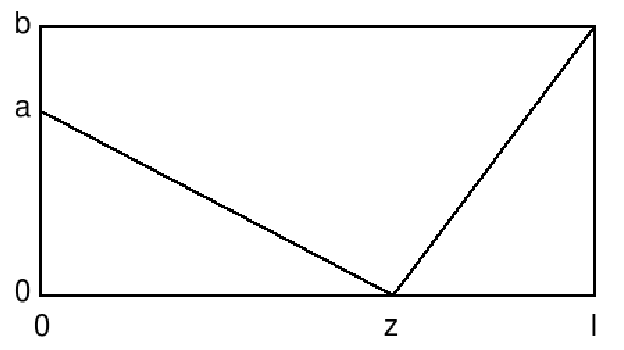
\includegraphics[width=2in]{trap}}

\caption{Generalized \emph{l-trap} function. }
\label{fig:trap}
\end{figure}
%%%%%%%%%%%%%%%%%%%%%%%%%%%%%%%%%%%


For the following experiments, 2-trap, 3-trap and 4-trap functions were designed with the following parameter values: $a = l-1$; $b = l$; $z = l-1$. With these settings, 2-trap  is not deceptive, 4-trap is deceptive and 3-trap lies in the region between deception and non-deception. Under these conditions, it is possible not only to examine how \emph{EvAg} scales on trap functions, but also to investigate how the scalability varies when changing from non-deceptive to deceptive search landscapes.
Scalability tests were performed by juxtaposing \textit{m}\ trap functions and summing the fitness of each sub-function to obtain the total fitness. 




The bisection method  \cite{sastry:bisection} was used for each trap and each size \textit{m}\ to determine
the optimal \emph{EvAg} population size P, that is, the lowest P for which
98\% of the runs solve the traps functions. To find it, mutation rate
is set to 0, so as to search a minimum population size such
that using random initialization it is able to provide enough building
blocks to converge to the optimum without other mechanism than
recombination and selection. 


Algorithm \ref{alg:bisection} depicts the method based on bisection.
The method begins with a small population size which is doubled until
the algorithm ensures a reliable convergence. We define the
reliability criterion as the convergence of the algorithm to the
optimum 49 out of 50 times (0.98 of Success Rate). After that, the
interval $(min,max)$ is halved several times and the population size
adjusted within such a range. $min$ and $max$ stand respectively for the minimum and maximum population size estimated.

%%%%%%%%%%%%%%%%%%%%%%
\begin{algorithm}
\caption{Method based on Bisection}
\label{alg:bisection}
\begin{algorithmic}
\STATE P = Initial Population Size
\WHILE{ Algorithm reliability $<$ 98\%}
\STATE min = P ; max, P = Double (P)
\ENDWHILE
\WHILE{ $\frac{max-min}{min} > \frac{1}{16}$}
\STATE $P = \frac{max+min}{2}$ 
\STATE (Algorithm reliability $<$ 98\%) ? min = P : max = P
\ENDWHILE
\end{algorithmic}
\end{algorithm}
%%%%%%%%%%%%%%%%%%%%%%






%%%%%%%%%%%%%%%%%%%%%%%%%%%%%%%%%%%
\begin{figure}[!htpb]
\centerline{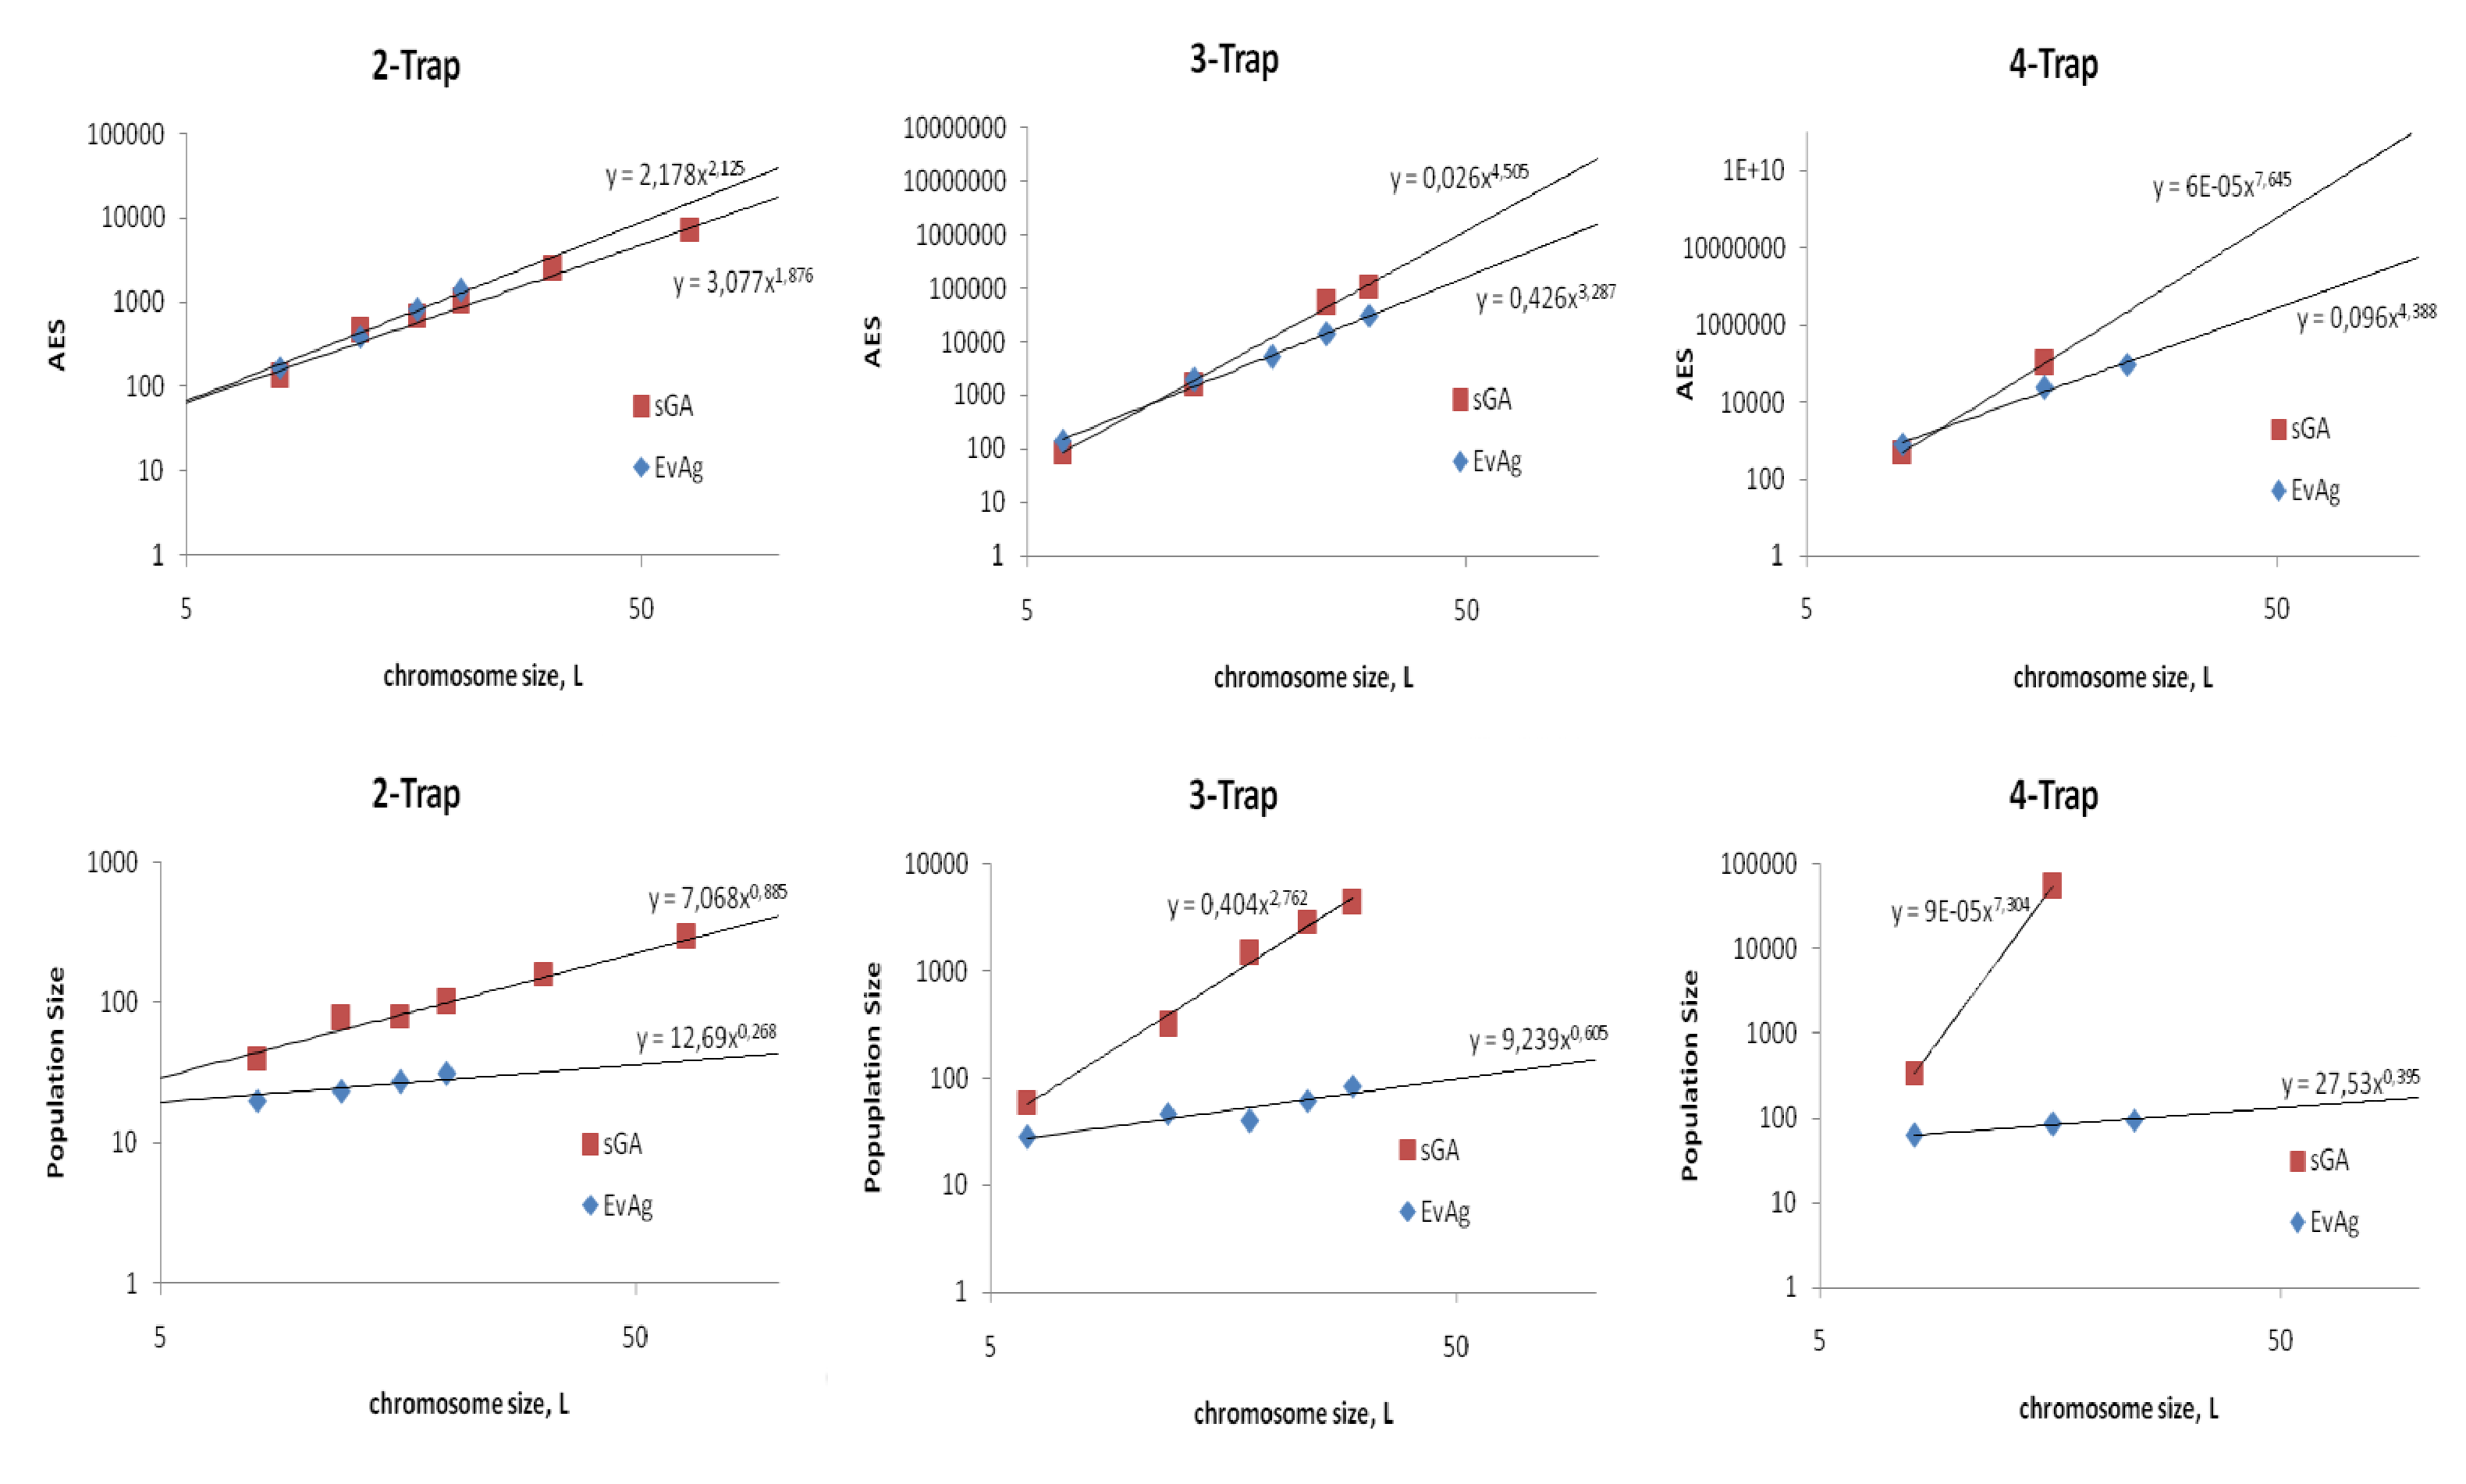
\includegraphics[width=5in]{scalability2}}

\caption{Scalability with trap functions. Optimal population size and Average Evaluations to Solution (AES) values for a standard GA (sGA) and the Evolvable Agent Model (EvAg). }
\label{fig:scalability}
\end{figure}
%%%%%%%%%%%%%%%%%%%%%%%%%%%%%%%%%%%

\emph{EvAg} was tested with $p_c = 1.0$, uniform crossover and binary tournament. Results are depicted in figure \ref{fig:scalability}.

From the graphics in figure \ref{fig:scalability} it can be concluded that \emph{EvAg} scales better than a standard GA on 2, 3 and 4-trap, but the improvement is much more noticeable when solving the deceptive 4-trap function. Under these conditions (4-trap), a standard GA faces extreme difficulties because lower order building blocks mislead the search towards local optima instead of combining to form higher order building-blocks, thus challenging the GA's search mechanisms, and if the problem size grows, the computational effort grows exponentially. A possible explanation for \emph{EvAg}'s better scalability lies in its ability to maintain genetic diversity at a higher and consequent reduction of its optimal population size (N). With a lower optimal N, \emph{EvAg} needs fewer evaluations to reach the optimum, when compared to standard GAs. 
